\documentclass[twoside]{article}
\usepackage[utf8]{inputenc}
\usepackage[spanish,es-noshorthands]{babel}
\usepackage[T1]{fontenc}
\usepackage{lmodern}
\usepackage{graphicx,hyperref}
\usepackage{tikz,pgf}
\usepackage{marvosym}
\usepackage{multicol}
\usepackage{fancyhdr}
\usepackage{framed}
\usepackage{color}
\usepackage{wrapfig}\definecolor{shadecolor}{RGB}{204,255,204}
\usepackage[papersize={8.5in,13in},total={7.5in,11.75in},centering]{geometry}
\usepackage{fancyhdr}
\pagestyle{fancy}
\fancyhead[LE]{IEDAB}
\fancyhead[RE]{PEI:``Hacia una cultura para el desarrollo sostenible''}
%\fancyfoot[RO]{\Email iedabgerman@autistici.org}
%\fancyhead[LO]{\url{www.autistici.org/mathgerman}}
% \fancyfoot[RE]{\Email iedabgerman@autistici.org}
% \fancyfoot[LE]{\url{www.autistici.org/mathgerman}}
 \fancyhead[RO]{IEDAB}

%\author{Germ\'an Avenda\~no Ram\'irez~\thanks{Lic. Mat. U.D., M.Sc. U.N.}}
\title{\begin{minipage}{.2\textwidth}

\includegraphics[height=1.75cm]{Images/logo-colegio.png}\end{minipage}
\begin{minipage}{.55\textwidth}
\begin{center}
GUÍA: PEDAGOGÍA SOBRE CONSULTA POPULAR DEL 26 DE AGOSTO DE 2018\\
\end{center}
\end{minipage}\hfill
\begin{minipage}{.2\textwidth}

\includegraphics[height=1.75cm]{Images/logo-sed.png} 
\end{minipage}}
\date{}
\thispagestyle{plain}
\begin{document}
\maketitle
\vspace{-.7in}
\fbox{
  \begin{minipage}{0.9\linewidth}
    \emph{Se realizará el día miércoles 22 de agosto de 2018 en las primeras 2 horas de clase  en primaria con acompañamiento del grado 1003 y en bachillerato las 2 últimas horas de clase con acompañamiento del grado 1103.}
    \end{minipage}
  }
\section*{Logros}
\begin{itemize}
\item Conocer e identificar  los mecanismos de participación ciudadana, en este caso la consulta popular anti-corrupción.
\item Conocer los siete puntos  que hacen parte de la consulta anti-corrupción. 
\end{itemize}
Según la Constitución Política de Colombia de 1991 en los artículos 1$^\circ$ y 2$^\circ$, Colombia es un “ESTADO SOCIAL DE DERECHO, ES DEMÓCRATICA, PARTICIPATIVA Y PLURALISTA”. El estado debe garantizar a través de la educación el cumplimiento de estos fines, para que la población colombiana tenga participación real en la toma de decisiones que afectan al país en lo económico, administrativo, político y cultural.De acuerdo al artículo 103 de la Constitución política de Colombia, Ley 134 del /94, son mecanismos de participación del pueblo en ejercicio de su soberanía: el voto, el plebiscito, referendo, cabildo abierto, iniciativa legislativa, revocatoria del mandato y consulta popular.

La consulta popular es un mecanismo de participación mediante el cual unas preguntas de carácter general sobre temas de trascendencia nacional, departamental, distrital, municipal y local son sometidas por el presidente de la república, el gobernador, el alcalde a consideración del pueblo para que este se pronuncie sobre ellas; en nuestro caso el 26 de agosto del presente año se realizara la consulta popular anticorrupción en Colombia con las siguientes preguntas:
\begin{enumerate}
  \begin{minipage}{0.5\textwidth}
  \item REDUCIR EL SALARIO DE LOS CONGRESISTAS Y ALTOS FUNCIONARIOS DEL ESTADO: ¿Aprueba usted reducir el salario de los congresistas de 40 a 25 salarios mínimos legales mensuales vigentes, fijando un tope de 25 (SMLV) como máxima remuneración mensual de los congresistas y altos funcionarios del estado, señalados en el artículo 197 de la constitución política?
  \end{minipage}\hfill
  \begin{minipage}{0.4\textwidth}
    \begin{shaded}
\emph{Mientras que el salario mínimo está en \$781\,242, la remuneración mensual de un congresista es de \$31'331\,821. Se calcula que entre salarios, primas sobresueldos, etc, de congresistas y altos funcionarios, el país se ahorraría cada año más de 200 mil millones de pesos por esta razón apoyamos la consulta. Vamos a votar SÍ.}
      \end{shaded}
    \end{minipage}
    \begin{minipage}{0.35\linewidth}
      \begin{shaded}
\emph{      A pesar de los escándalos de corrupción y robos al Plan de Alimentación Escolar (PAE), las empresas pudieron seguir manejando contratos y el llamado \textsc{``zar del PAE''} recibió el beneficio de ``casa por cárcel''}
    \end{shaded}
    \end{minipage}\hfill
    \begin{minipage}{0.6\linewidth}
  \item CÁRCEL A CORRUPTOS Y PROHIBIRLES CONTRATAR CON EL ESTADO ¿Aprueba usted que las personas condenadas por corrupción y delitos contra la administración pública deban cumplir la totalidad de las penas en la cárcel sin posibilidades de reclusión especial y que el estado unilateralmente pueda dar por terminados los contratos con ellas y con las personas jurídicas  de las que hagan parte, sin que haya lugar  a indemnización alguna por el contratista
  \end{minipage}
  \begin{minipage}{0.5\linewidth}
\item CONTRATACIÓN TRANSPARENTE OBLIGATORIA EN TODO EL PAÍS ¿Aprueba usted establecer la obligación a todas las entidades públicas y territoriales de usar pliegos tipo, que reduzcan la manipulación de requisitos habilitantes y ponderables y la contratación a dedo   con un número anormalmente bajo de proponentes, de todo tipo de contrato con re cursos públicos     
\end{minipage}\hfill
\begin{minipage}{0.45\linewidth}
  \begin{shaded}
\emph{  Esto es muy importante, pues más del 80\% de los contratos estatales se hacen de forma directa o mediante licitaciones en la que participa un solo proponente; son cerca de 70 billones al año que se estarían entregando sin cumplir las reglas de la contratación pública.}
\end{shaded}
\end{minipage}
\begin{minipage}{0.45\linewidth}
  \begin{shaded}
    \emph{ \$84 billones es el Presupuesto de Inversión de la Nación en este año 2018. Gran parte de estos recursos deberían ser priorizados con participación ciudadana. Fuente: La Nación /oct.20/2017\\
    Con esta pregunta de la consulta se promueven dos principios: la participación ciudadana y la transparencia en el proceso presupuestal. Votaré sí en la consulta }
  \end{shaded}
\end{minipage}\hfill
\begin{minipage}{0.5\linewidth}
\item PRESUPUESTOS PUBLICOS CON PARTICIPÀCIÓN DE LA CIUDADANÍA ¿Aprueba usted establecer la obligación de realizar audiencias públicas para que la ciudanía y los corporados decidan el desglose y priorización del presupuesto de inversión de la nación, los departamentos y los municipios, así como la rendición de cuentas  sobre su contratación y ejecución. 
\end{minipage}
\begin{minipage}{0.55\linewidth}
\item CONGRESISTAS DEBEN RENDIR CUENTAS DE SU ASISTENCIA, VOTACIÓN Y GESTIÓN ¿Aprueba usted obligara a congresistas y demás corporados a rendir cuentas anualmente sobre su asistencia, iniciativas presentadas, votaciones, debates, gestión de intereses particulares o de lobbistas, proyectos partidas e inversiones públicas que haya gestionado y cargos públicos para los cuales hayan presentado candidatos?
\end{minipage}\hfill
\begin{minipage}{0.4\linewidth}
  \begin{shaded}
    \emph{Con nuestro SÍ en la consulta anti-corrupción lograremos que los políticos que elijamos al congreso se vean obligados a RENDIR CUENTAS, de lo que hacen. Así, se hace más transparente su labor parlamentaria .Así, los ciudadanos podemos juzgar que tan conveniente es volver a elegirlos.}
  \end{shaded}
\end{minipage}
\begin{minipage}{0.6\linewidth}
\item HACER PÚBLICAS LAS PROPIEDADES E INGRESOS INJUSTIFICADOS DE POLÍTICOS Y EXTINGUIRLES EL DOMINIO ¿Aprueba usted obligar a todos  los electos mediante voto popular a hacer públicas a escrutinio de la ciudadanía sus declaraciones de bienes ,  patrimonio, rentas, pago de impuestos y conflictos de interés, requisito para posesionarse y ejercer el cargo; incorporando la facultad  de iniciar de oficio investigaciones penales y aplicar la extinción de dominio al elegido y a su potencial red de testaferros como su cónyuge, compañero(a) permanente, a sus parientes dentro del 4 grado de consanguinidad, segundo de afinidad y primero civil y a sus socios de derecho o de hecho
\end{minipage}\hfill
\begin{minipage}{0.35\linewidth}
  \begin{shaded}
  \emph{La mayoría de congresistas se ha opuesto a esta iniciativa y ha bloqueado los proyectos que buscan darle transparencia a sus ingresos.
Muchas veces los políticos recurren a familiares o amigos cercanos  para poner a su nombre propiedades que han logrado.}
\end{shaded}
\end{minipage}
\begin{minipage}{0.4\linewidth}
  \begin{shaded}
    \emph{Tres periodos máximo es justo; el que quieres servir y tiene iniciativas puede hacer una labor en doce años, si participamos con el SÍ en la consulta anticorrupción los políticos de profesión solo podrán estar en una corporación pública máximo tres períodos. }
  \end{shaded}
\end{minipage}\hfill
\begin{minipage}{0.55\linewidth}
\item NO MÁS ATORNILLADOS EN EL PODER : MÁXIMO TRES PERÍODOS EN CORPORACIONES PUBLICAS ¿Aprueba usted establecer un límite de máximo de tres periodos para ser elegido y ejercer en una misma corporación de elección popular como el senado de la república, la cámara de representantes las asambleas departamentales, los concejos municipales y las juntas administradoras locales?
\end{minipage}
\end{enumerate}

\section*{Mentiras y verdades sobre la consulta}

\begin{minipage}{0.45\linewidth}
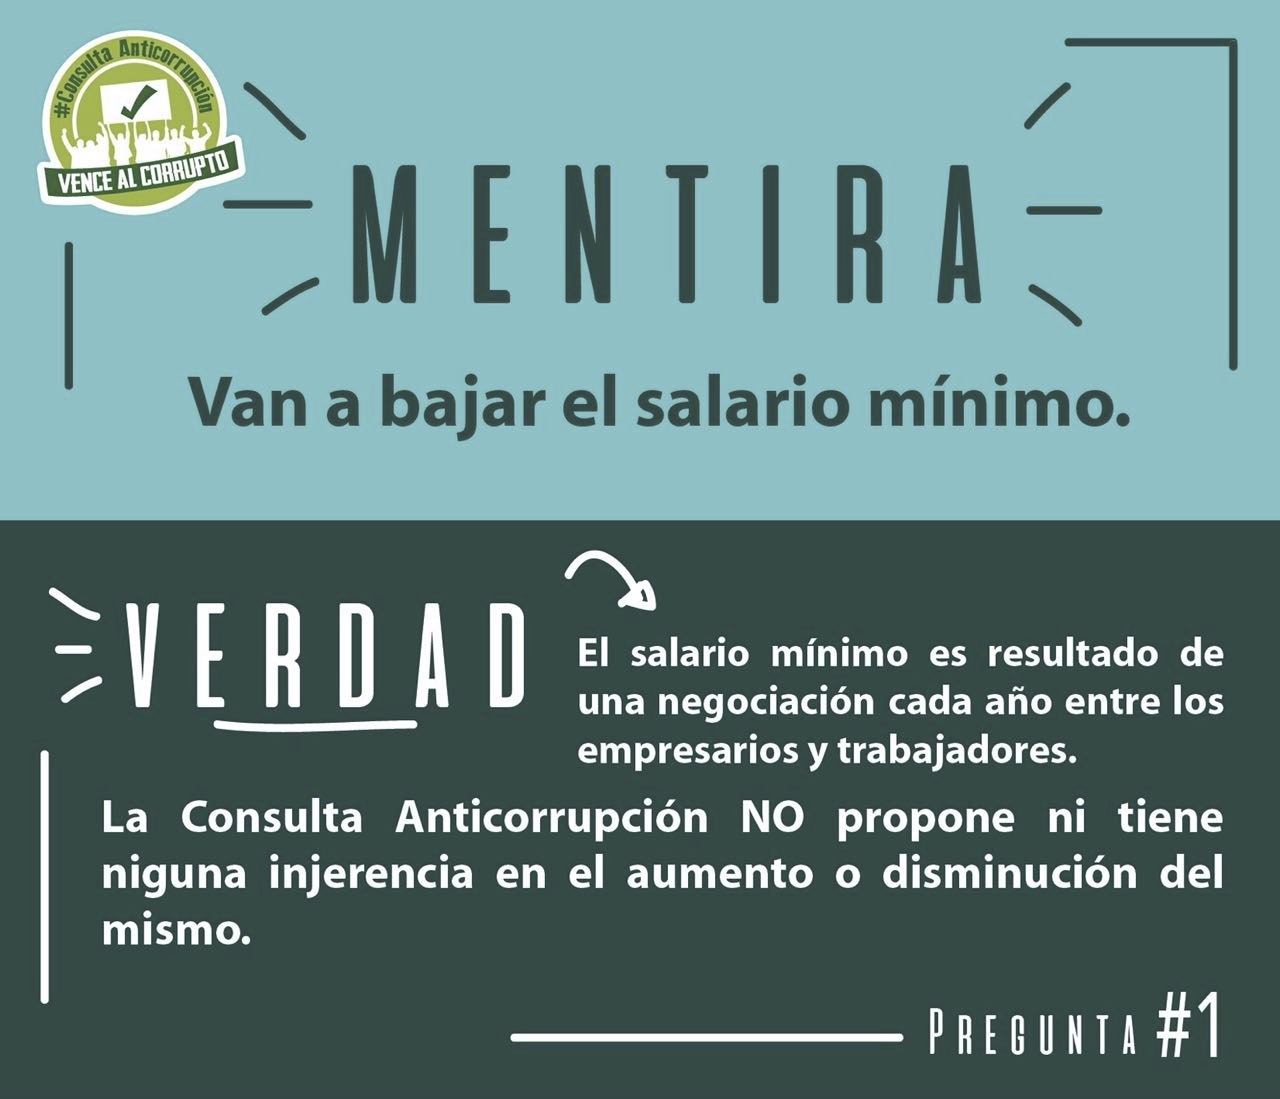
\includegraphics[scale=.175]{Images/mentira_consulta_anticorrupcion_salario_minimo.jpeg}
\end{minipage}\hfill
\begin{minipage}{0.45\linewidth}
  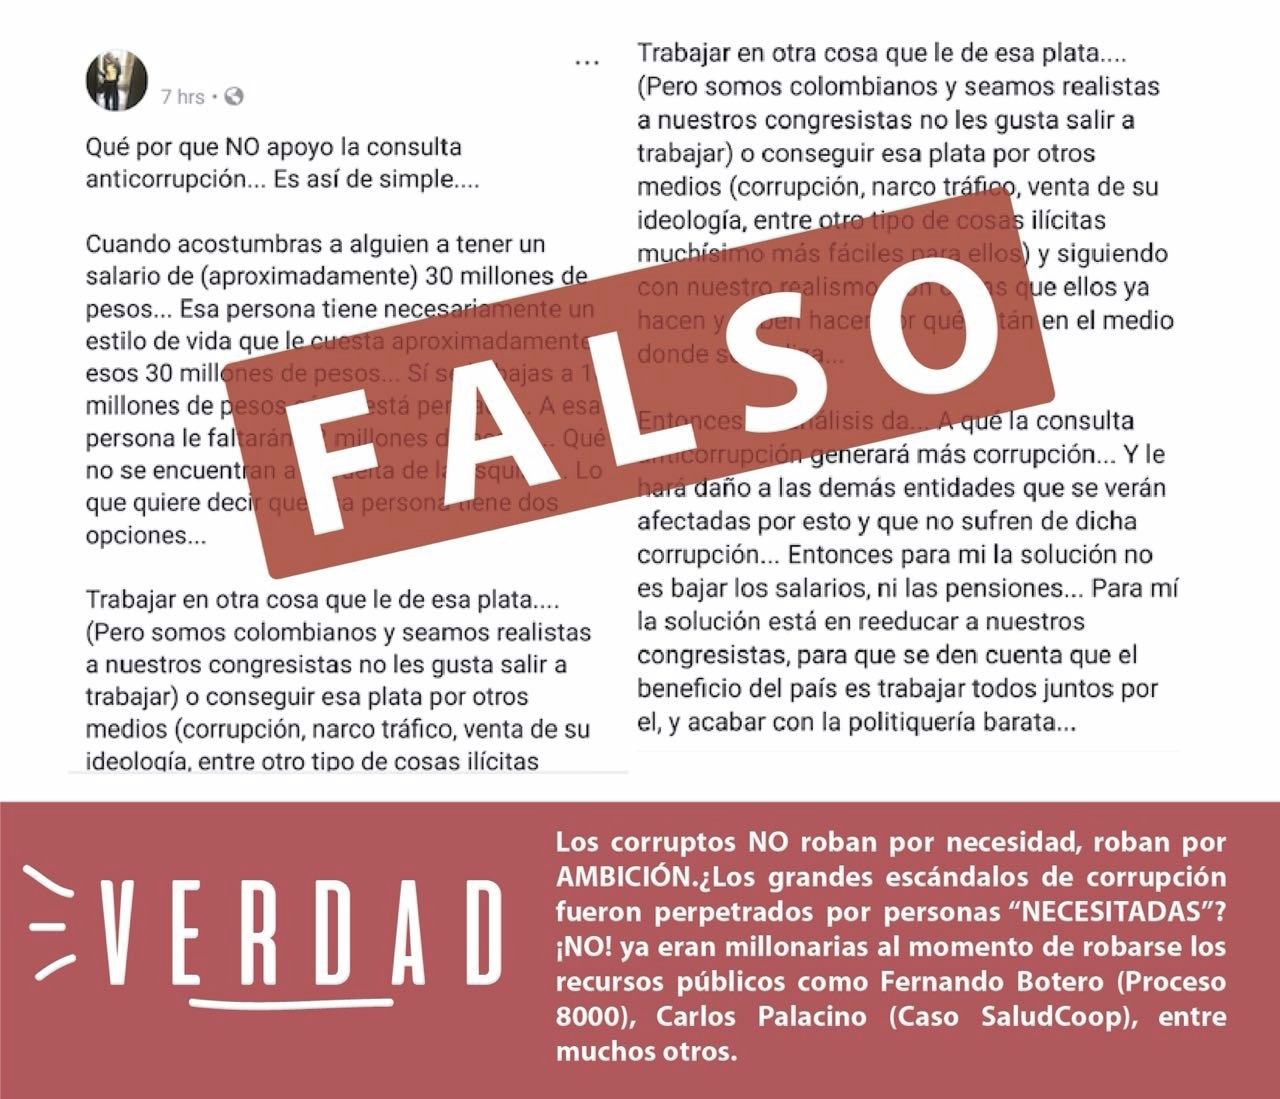
\includegraphics[scale=.175]{Images/mentira_consulta_anticorrupcion_salario_congresistas_estilo_vida.jpeg}
\end{minipage}
\begin{minipage}{0.45\linewidth}
  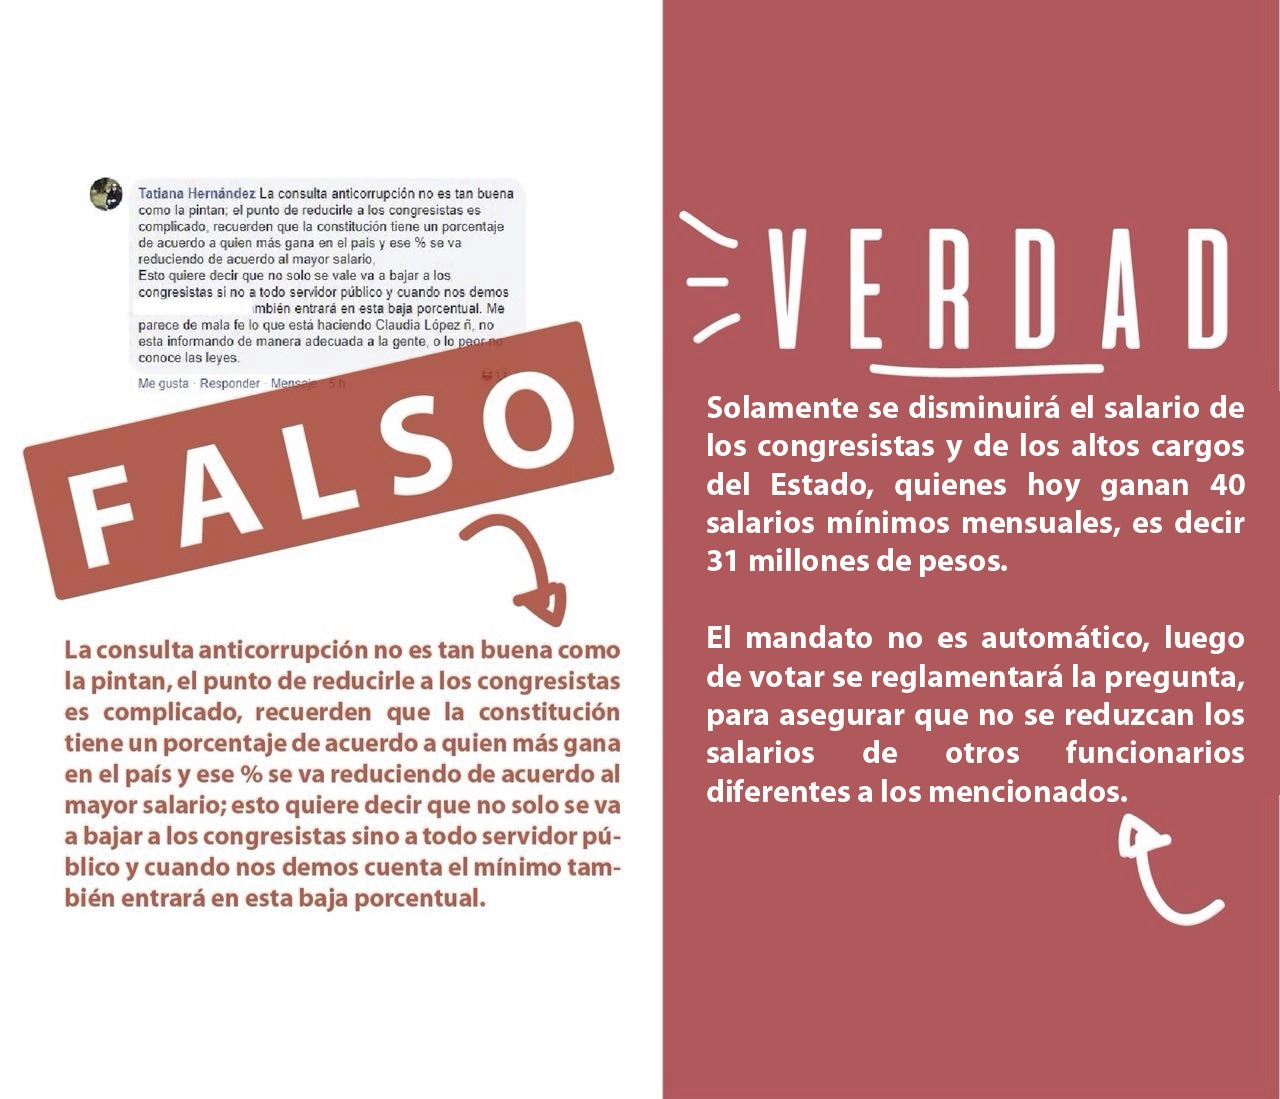
\includegraphics[scale=.175]{Images/mentira_consulta_anticorrupcion_salario_congresitas.jpeg}
\end{minipage}\hfill
\begin{minipage}{0.45\linewidth}
  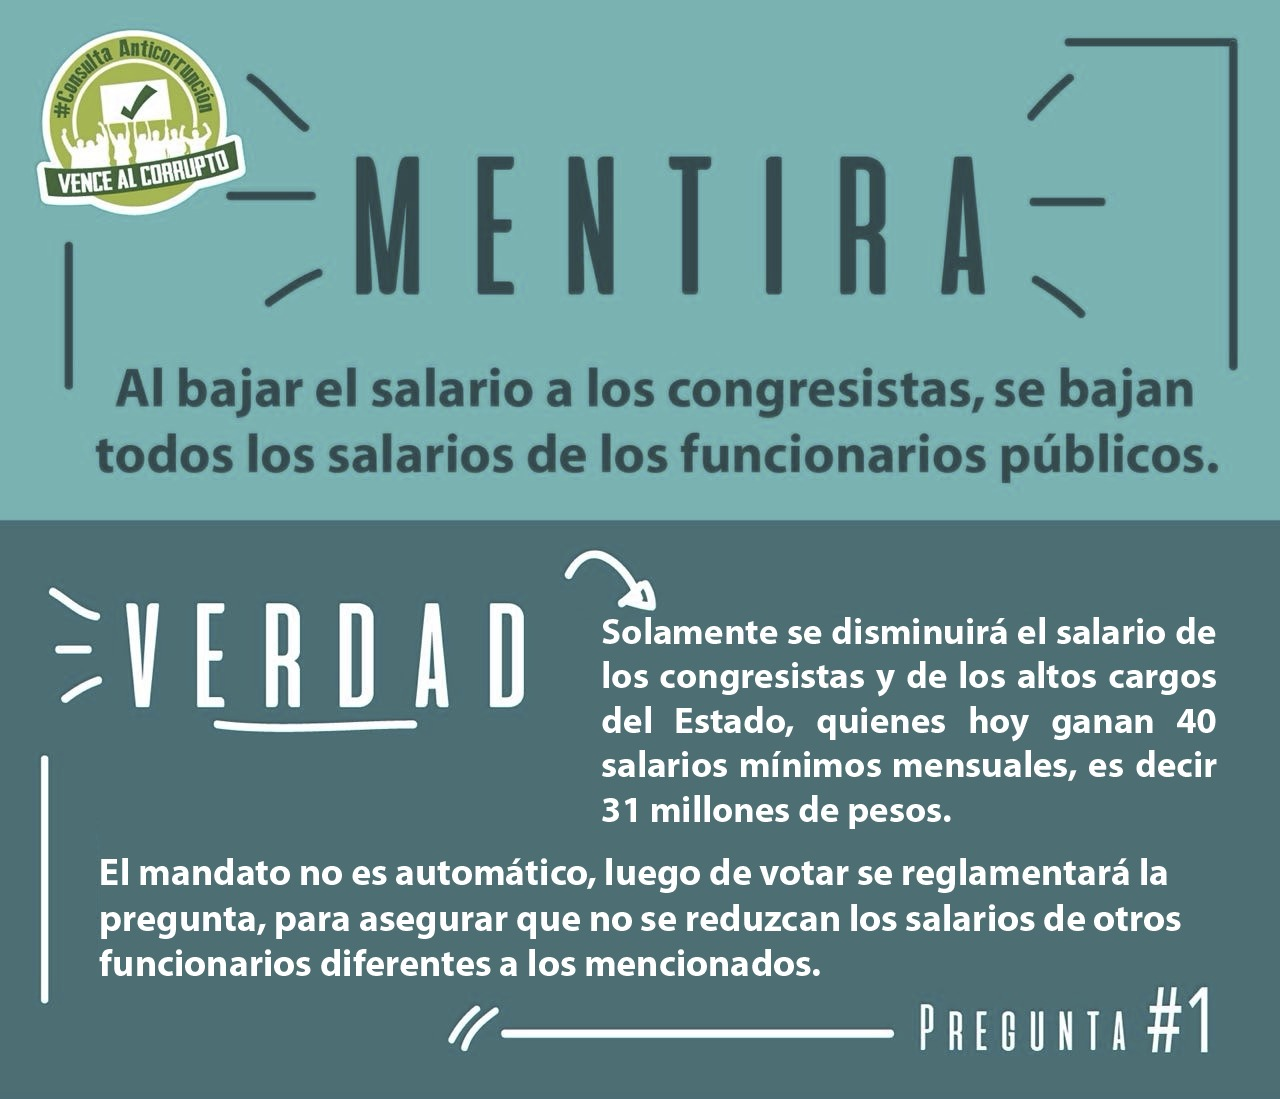
\includegraphics[scale=.175]{Images/mentira_consulta_anticorrupcion_salario_funcionarios_publicos.jpeg}
\end{minipage}

\section*{ACTIVIDAD}
\begin{enumerate}
\item Después de hacer lectura de la guía y tener en cuenta la explicación de los estudiantes de grado décimo y once, anotar las siete preguntas en el cuaderno de ecología  o matemáticas y escribir algunas razones por las que se debe votar SÍ.
\item Identificar qué mecanismos de participación  ciudadana nos ha dado la constitución política de Colombia de 1991 y consulte en qué consiste cada uno, de tarea en su casa.
\item Hable con sus acudientes y explíqueles las razones por las cuales es muy importante salir a votar el domingo 26 de agosto de 2018 la Consulta Anti-corrupción, con el propósito de que el presupuesto del país sea bien invertido, con ayuda de la participación democrática de todos los colombianos.
\item Consulte en la página \url{www.vencealcorrupto.com} otras ``fake-news'' para que pueda aclararle a otras personas cuando escuchen o reciban mensajes por redes sociales con noticias falsas.
\item Consulte la Cartilla Anticorrupción que hizo Fecode, para que pueda tener más elementos de análisis al respecto. \url{http://www.fecode.edu.co/images/comunicados/2018/CartillaAntiCorrupcion.pdf}
\item Con tres compañeros más, haga una cartelera alusiva a la \emph{Consulta Anticorrupción}
\end{enumerate}
\end{document}
